\documentclass[spanish]{article}
\usepackage[utf8]{inputenc}
\usepackage{babel}
\usepackage{multirow}
\usepackage{graphicx}
\usepackage{float}
\usepackage{enumerate}
\usepackage{lmodern}
\usepackage[T1]{fontenc}
\usepackage{mathtools}
\usepackage[usenames,dvipsnames]{xcolor}
\usepackage{graphicx}
\usepackage{lscape} 
\usepackage{pdflscape} 
\usepackage{fancyvrb}
\usepackage{listings}
\usepackage{fancybox}
\usepackage{listings}
\definecolor{light-gray}{gray}{0.85}
\definecolor{mimalva}{rgb}{0.58,0,0.99}

   \lstset{
	basicstyle=\normalsize\ttfamily,     
	numbers=left,               
	language=c,
	stepnumber=1,               
	numbersep=1em,              
	aboveskip=1em,
	keepspaces=false,      
	showstringspaces=false,        
	belowskip=0.2em,
	keywordstyle=\ttfamily\color{ForestGreen}\bfseries,
		stringstyle=\color{RubineRed}, 
        %identifierstyle=\ttfamily\color{Sepia}\bfseries,
        commentstyle=\color{NavyBlue},
        morecomment=[l][\color{Periwinkle}]{\#},
	backgroundcolor=\color{white},
	numberstyle=\footnotesize\color{Gray},
	frame=single,
	rulecolor=\color{NavyBlue},
    }

\title{Migración y optimización del sistema Proceso Electoral.}


\author{Katherine Andrade.}

%si quieres quitar la fecha descomentas la linea de abajo
\date{}


\begin{document}


\begin{figure}
	\centering
	
\includegraphics[width=0.99\textwidth]{Logo_computacion}
\end{figure}


\maketitle

\section{Capitulo I}

\subsubsection{Marco de Referencia}
Ogangi de Venezuela, C.A entrega millones de transacciones a través de las redes de
datos móviles de América a través de su plataforma y actualmente procesa más de un millón de
mensajes diarios, con sistemas informáticos redundantes, tolerante a fallas y con soporte las 24
horas del día, por 7 días a la semana, los 365 días del año.

\subsubsection{Misión:}
Su Misión está representada por la siguiente afirmación:
“La tecnología de software y propiedad intelectual de Ogangi acelera y facilita la evolución
de servicios móviles de datos. Permite a los operadores celulares crecer más rápidamente su
oferta de servicios, a los proveedores y dueños de contenido de crear una presencia móvil, y a
los usuarios móviles de gozar de los servicios a través de una experiencia satisfactoria”.

\subsubsection{Visión:}
“Los teléfonos, redes y servicios de datos de la telefonía móvil continuarán madurando y
evolucionando hasta consolidarse como un medio de comunicación más comparable a los
medios tradicionales como televisión y más recientemente Internet. La conveniencia de la
ubicuidad y flexibilidad de los servicios móviles de datos permitirá a este nuevo medio inclusive
integrar varios de los tradicionales”. \\

En la actualidad, el negocio de Ogangi se divide principalmente en tres areas:

\begin{itemize}
	
	\item Mensajería corporativa.	 
	\item Descarga de contenidos por medio de portales WAP y WEB. 	 
	\item Desarrollo de aplicaciones móviles. 	 
\end{itemize}

De las tres áreas mencionadas, la mensajería corporativa ha sido el negocio principal de Ogangi desde sus inicios. Es por eso que año tras año, y juntos con los avances tecnológicos y tendencias en el mercado, Ogangi ha ido enriqueciendo su plataforma de mensajería, ofreciendo a sus clientes cada vez más canales para la entrega de información. \\

Ogangi cuenta con una solución de mensajería interactiva que le permite a los usuarios obtener información referente al votante en un proceso electoral. \\
Básicamente el cliente(compañía, empresa, etc) encargado del proceso proporciona los datos de los votantes a Ogangi, los cuales son insertados en una base de datos a través de un script, para ser consultados via SMS por los votantes.

Las pasantias fueron realizadas especificamente en el area de desarrollo. Donde se realizo la actualización del proyecto que hace posible el envio de mensajes para obtener información referente al votante en un proceso electoral.

\section{Capitulo II}

\subsection{Bases Teoricas:}

\subsubsection{Programación Orientada a Objetos:}

La programación orientada a objetos es un paradigma de programación que usa los objetos en sus interacciones, para diseñar aplicaciones y programas informáticos. \\
%https://es.wikibooks.org/wiki/Programaci%C3%B3n_Orientada_a_Objetos

Los objetos son entidades que combinan estado (atributo), comportamiento (método) e identidad.

El estado de un objeto se refiere al conjunto de atributos y sus valores en un instante de tiempo dado. El comportamiento de un objeto puede modificar el estado de este.
%https://es.wikipedia.org/wiki/Objeto_(programaci%C3%B3n)#Estado
\\
El comportamiento de un objeto, está directamente relacionado con su funcionalidad y determina las operaciones que este puede realizar o a las que puede responder ante mensajes enviados por otros objetos. \\

La identidad, es la propiedad que permite diferenciar a un objeto y distinguirse de otros. Generalmente esta propiedad es tal, que da nombre al objeto \\

Este tipo de programación, está basada en varias técnicas, incluyendo herencia, cohesión, abstracción, polimorfismo, acoplamiento y encapsulamiento.

Su uso se popularizó a principios de la década de los años 1990. En la actualidad, existe variedad de lenguajes de programación que soportan la orientación a objetos.

\subsection{JAVA:} 

Java es un lenguaje de programación orientado a objetos y es multiplataforma, ya que se puede ejecutar un mismo codigo en cualquier SO gracias a que se utiliza un entorno de ejecucion de JAVA llamado JRE.
Este lenguaje fue desarrollado por Sun Microsystems, posteriormente adquirido por Oracle. En la actualidad puede utilizarse de modo gratuito, pudiéndose conseguir sin problemas un paquete para desarrolladores que oriente la actividad de programar en este lenguaje. \\

 Puede ser modificado por cualquiera, circunstancia que lo convierte en lo que comúnmente se denomina “código abierto”.

... Via Definicion.mx: https://definicion.mx/java/


\subsection{Procedimientos almacenados:}

Un procedimiento almacenado es un programa almacenado fisicamente en una base de datos.
Este programa al ser ejecutado en respuesta a una peticion de usuario, es ejecutado directamente en el motor de la base de datos, el cual usualmente corre en un servidor separado. Como tal, posee acceso directo a los datos que necesita manipular y sólo necesita enviar sus resultados de regreso al usuario, deshaciéndose de la sobrecarga resultante de comunicar grandes cantidades de datos salientes y entrantes. \\

La mayor parte de las veces, se utilizan para encapsular procesos complejos que podrían requerir  la ejecución de varias consultas SQL, tales como la manipulación de un conjunto de datos enorme para producir un resultado resumido. \\

También pueden ser usados para el control de gestión de operaciones, y ejecutar procedimientos almacenados dentro de una transacción de tal manera que las transacciones sean efectivamente transparentes para ellos. \\

La ventaja de un procedimiento almacenado, en respuesta a una petición de usuario, está directamente bajo el control del motor del gestor de bases de datos, que corre generalmente en un servidor distinto del servidor web, aumentando con ello la rapidez de procesamiento de las peticiones del usuario. El servidor de la base de datos tiene acceso directo a los datos necesarios para manipular y sólo necesita enviar el resultado final al usuario. Los procedimientos almacenados pueden permitir que la lógica del negocio se encuentre como un API en la base de datos, que pueden simplificar la gestión de datos y reducir la necesidad de codificar la lógica en el resto de los programas cliente. Esto puede reducir la probabilidad de que los datos se corrompan por el uso de programas clientes defectuosos o erróneos. De este modo, el motor de base de datos puede asegurar la integridad de los datos y su consistencia con la ayuda de procedimientos almacenados.
%https://es.wikipedia.org/wiki/Procedimiento_almacenado


\subsection{Hibernate:}

Hibernate es una herramienta de Mapeo objeto-relacional, esto quiere decir, que facilita el mapeo de atributos entre una base de datos relacional tradicional y el modelo de objetos de una aplicación, mediante archivos declarativos (XML) o anotaciones en los beans de las entidades que permiten establecer estas relaciones. \\
Está diseñado para ser flexible en cuanto al esquema de tablas utilizado, para poder adaptarse a su uso sobre una base de datos ya existente. También tiene la funcionalidad de crear la base de datos a partir de la información disponible. \\

Hibernate es software libre, distribuido bajo los términos de la licencia GNU LGPL

http://blog.educacionit.com/2013/02/07/que-es-java-hibernate/

https://es.wikipedia.org/wiki/Hibernate


\subsection{Sistema de Gestor de Base De Datos(SGBD):}

es un conjunto de programas no visibles que administran y gestionan la información que contiene una base de datos. A través de él se maneja todo acceso a la base de datos con el objetivo de servir de interfaz entre ésta, el usuario y las aplicaciones.

En este proyecto, se utilizaron dos SGBD los cuales fueron: Oracle y Postgresql.

Oracle, es un sistema de gestión de base de datos relacional (o RDBMS por el acrónimo en inglés de Relational Data Base Management System), fabricado por Oracle Corporation.
\\
 Tradicionamente Oracle ha sido el SGBS por excelencia, considerado siempre como el más completo y robusto. ambien siempre ha sido considerado de los más caros, por lo que no se ha estadarizado su uso como otras aplicaciones.
 
 Postgresql, es un sistema de gestión de base de datos relacional orientada a objetos y libre, publicado bajo la licencia BSD.
 
 Como muchos otros proyectos de código abierto, el desarrollo de PostgreSQL no es manejado por una empresa y/o persona, sino que es dirigido por una comunidad de desarrolladores que trabajan de forma desinteresada, libre y/o apoyada por organizaciones comerciales. La comunidad PostgreSQL se denominada el PGDG (PostgreSQL Global Development Group).
 
% https://revistadigital.inesem.es/informatica-y-tics/los-gestores-de-bases-de-datos-mas-usados/

\section{Capitulo III:}

\subsection{Aspectos Procedimentales:}

\subsubsection{Plan de trabajo:}

\begin{figure}[htb]
	\centering
	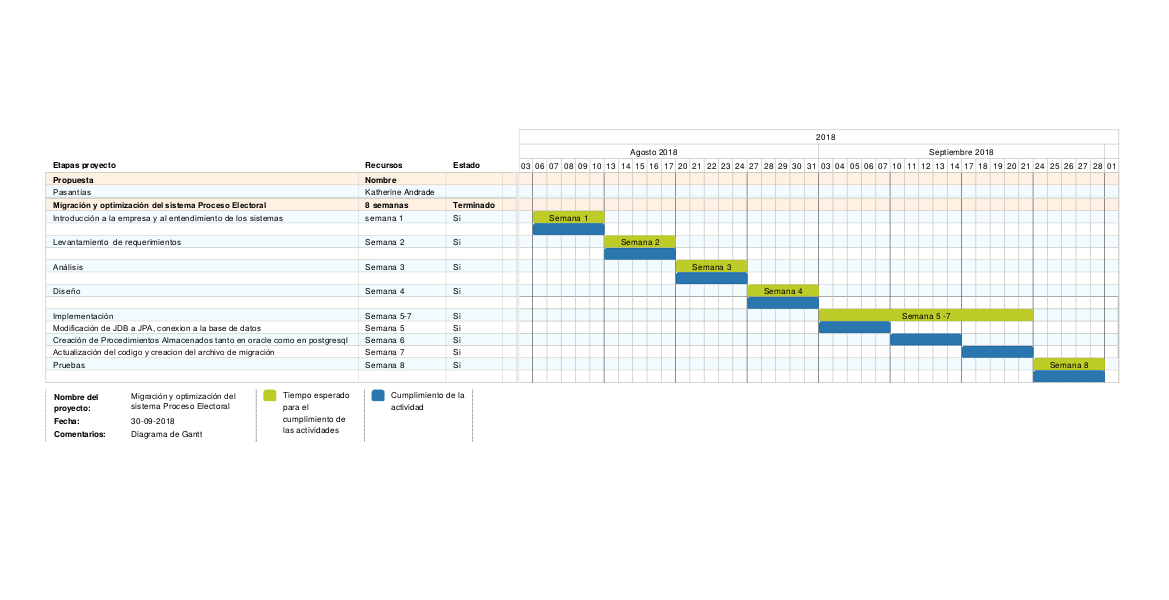
\includegraphics[width=1\textwidth]{diagrama1.png}
	\caption{Diagrama de Gantt}
	\label{i1}
\end{figure}


\subsection{Introducción a la empresa y al entendimiento de los sistemas:}
Semana dedicada a la introducción sobre la implementacion actual del sistema, presentada por el Lider de desarrollo José Hidalgo. Explicación del Proyecto que se va a actualizar. \\
Entrega de una computadora en la cual se realizara dicho proyecto.
Instalación de los diferentes proyectos y herramientas a utilizar. \\
Pruebas simples de las diferentes herramientas necesarias para poder llevar a cabo el proyecto de pasantias, con el fin de entender bien el manejo de dichas herramientas.

\subsection{Levantamiento de Requerimientos:}
Lograr el funcionamiento del proyecto basado en una conexión JPA. Crear las entidades en Hibernate cpn el fin de facilitar la migración de la base de datos, ya que hibernate permite la migración a cualquier gestor de base de datos. 

Creación de las entidades en Hibernate. Se selecciono una clave primaria para cada entidad, ya que a pesar de que la BD original es relacional, esta no contaba con las mismas. \\
Hibernate no permite crear entidades sin claves primarias. \\
 Para la mayoría de las tablas se escogió una clave primaria autoincremental.
 
Creación del archivo XML para poder realizar el mapeo. 

 
\subsection{Analisis:}
Modificación de las funciones que se encuentran en la clase CNEUtil, las cuales son las utilizadas para realizar las consultas a la BD que se encuentra en Oracle por medio de una conexión JDBC.Estas fueron modificadas a JPA y su conexión se realiza por medio de Hibernate. \\

Creación de Procedimientos Almacenados en Oracle de las consultas que se realizaban por medio de JDBC. 

Comienzo de la clase con la cual se realizara la migración de Oracle a Postgresql.

\subsection{Diseño:}

Creación de las tablas en Postgresql por medio del mapeo objeto-relacional. Esta creación se hizo en el servidor local. También se realizó la creación de los mismos Procedimientos Almacenados que se encuentran en Oracle, ya que estos funcionan correctamente.  

Culminación de la clase Migrate, la cual es la encargada de realizar la migración de Oracle a Postgresql.

\subsection{Implementación:}

Modificación de las funciones de las clases Updater y getDBDataTest. Cambio de JDBC a JPA. Las consultas se realizarón por medio de Procedimientos almacenados.\\
 
La clase Updater consta de funciones encargadas de insertar valores en una tabla especifica, actualizar o eliminar valores repetidos de la misma. La clase getDBDataTest hace una busqueda en la BD de una cedula con el fin de probar que la conexión es exitosa.

\subsection{Pruebas:}

Envío de un mensaje de texto para probar el funcionamiento del proyecto conectado con la BD remota que se encuentra en Oracle.
  
Realización de la migración de Oracle a Postgresql.


 

	
\end{document}